% CV.tex
% !TEX TS-program = pdflatex
% !TEX encoding = UTF-8 Unicode
\documentclass[9pt, oneside, a4paper, titlepage]{extarticle}

\usepackage[most]{tcolorbox}
\usepackage{tikz}
\usepackage{graphicx}
\usepackage[]{geometry}
\usepackage{booktabs}
\usepackage{setspace}
\usepackage{multicol}
\usepackage{hyperref}
\geometry{
    a4paper,
    left=0.1cm,
    right=0.1cm,
    top=0.2cm,
    bottom=0.1cm
    }
    \renewcommand{\baselinestretch}{0.95}
    \definecolor{titleBack}{RGB}{0,128,255} % Blue
    
    \title{Tobias SAVARY}
    \date{}
    
    \begin{document}

    % Create the rectangle at the top of the CV 
    \tcbset{colframe=gray!95!black, colback=titleBack, arc = 3mm}
    
    \begin{tcolorbox}
        % Use to fill in the top
        \begin{minipage}{0.3\linewidth}
            %This is the place for the picture of your face
            % \hspace*{-0.3cm}\includegraphics[scale = 0.5]{img/TOBIAS SAVARY Photo identité Oct2020.jpg}
            \hspace*{1cm}
            \begin{tikzpicture} 

                \begin{scope}
                    \clip [rounded corners=.5cm] (0,0) rectangle coordinate (centerpoint) (3.5,5cm); 
                    \node [inner sep=0pt] at (centerpoint) {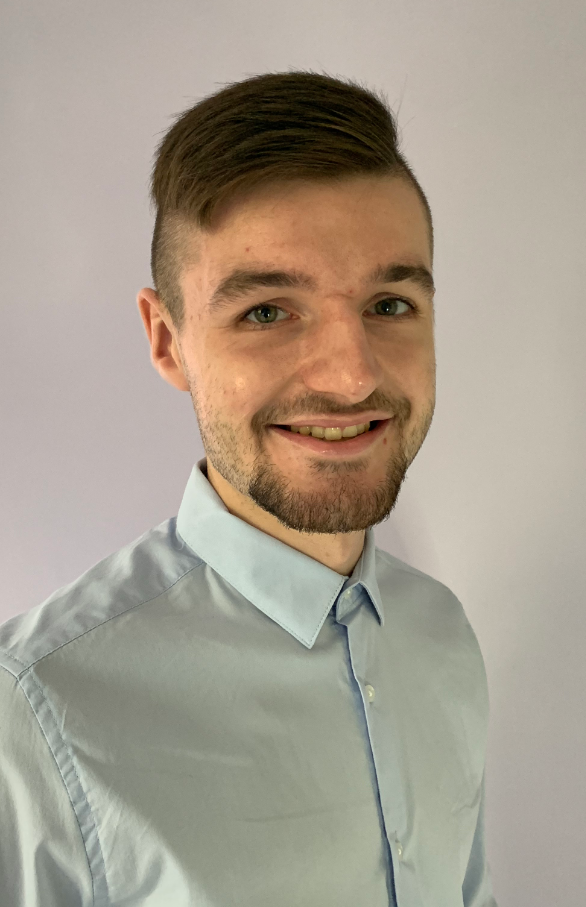
\includegraphics[width=3.5cm]{img/PhotoCV.png}}; 
                \end{scope}
            \end{tikzpicture}
        \end{minipage}%
        \hspace{1cm}%%
        \begin{minipage}{0.6\linewidth}
            \begin{center}
                \Huge{\textcolor{white}{Tobias SAVARY}} \\
                \vspace*{0.5cm}
                \Large{\textcolor{white}{\emph{Etudiant en Génie Informatique \\Université de Technologie de Compiègne (UTC) \\}}}
                \vspace*{0.5cm}
                \Large{\textcolor{white}{\emph{Recherche d'un stage de 6 mois \\en tant qu'assistant ingénieur en septembre 2023}}}
            \end{center}
        \end{minipage}%
    \end{tcolorbox}

    \tcbset{colframe=white, colback=white, arc = 2mm}
    \begin{tcolorbox}
        \vspace*{0.2cm}
        \hspace*{0.7mm}
        \begin{minipage}[t]{6.2cm}
            \begin{spacing}{0.95}
            \vspace*{-0.5cm}
            \begin{tcolorbox}[grow to left by = 0.6cm, colback = gray!25, colframe = white]
                % \section*{Profile}
                %     Here you can see my profile and I will complete it next time.
                
                \section*{\\Coordonnées}
                \hspace*{0.4cm}
                10 Bis Rue de Chateau Rouge

                \hspace*{0.4cm}
                \vspace*{0.2cm}
                60730 Cauvigny\\
                \hspace*{0.4cm}
                Tel: 07 65 21 77 91\\
                \hspace*{0.4cm}
                Email: savarytobias@hotmail.com\\
                \hspace*{0.4cm}
                \href{www.linkedin.com/in/tobiassavary}{www.linkedin.com/in/tobiassavary}
                \vspace*{0.2cm}

                \section*{Programmation}
                \begin{multicols}{2}
                    \begin{itemize}
                        \item Python
                        \item C
                        \item C++
                        \item SQL
                        \item Ocaml
                        \columnbreak                    
                        \item Lisp
                        \item ARM
                        \item HTML
                        \item CSS
                        \item \LaTeX
                    \end{itemize}
                    \end{multicols}
                    \vspace*{0.2cm}
                \section*{Compétences}

                \begin{itemize}
                    \vspace*{0.3cm}
                    \item Utilisation aisée des logiciels bureautiques (Word / Excel / Paint/ \\PowerPoint / \LaTeX \ldots)
                    \vspace*{0.2cm}
                    \item Utilisation aisée d’applications \\mobiles diverses
                    \vspace*{0.2cm}
                    \item Maîtrise des langages de programmation: Python, C, C++, SQL, Ocaml, Lisp, ARM, HTML, CSS\\
                    \vspace*{0.2cm}
                    \item Permis de conduire (Permis B)
                \end{itemize}


                \vspace*{0.2cm}
                \section*{Activités et intérêts}

                \begin{itemize}
                    \vspace*{0.3cm}
                    \item Participation aux manifestations de communication proposées par l’école (Journées Portes Ouvertes, Journée du lycéen, présentation de la formation auprès des élèves de Terminal dans les lycées de l’agglomération);
                    \vspace*{0.1cm}
                    \item Cyclisme: participation à divers évènements et rencontres sportives
                    \vspace*{0.1cm}
                    \item Natation, Badminton, 
                    
                    Tennis de Table
                    
                \end{itemize}

            \end{tcolorbox}
        \end{spacing}
        \end{minipage}
        \hspace*{0.4mm}
        \begin{minipage}[t]{12.8cm}
            \vspace*{-0.5cm}
            \begin{tcolorbox}[grow to right by = 0.6cm, colback = gray!25, colframe = white]
                \section*{Projets informatiques réalisés}
                \begin{itemize}
                    \item Réalisation de jeux de plateau en Python (scrabble, Futoshiki)
                    \item Gestion d’ensembles mathématiques en Ocaml
                    \item Traitement d’arbres phylogénétiques, décodage de message crypté, déplacement d’un robot, simplification de contours d’images en C
                    \item Codage de divers petites pages web avec HTML et CSS
                    \item Programmation orientée objet en C++ : conception et développement du jeu de société Machi Koro

                    \item Conception et réalisation d'une base de données pour une clinique vétérinaire en SQL avec une interface Python
                    
                    \item Réalisation d'un système expert en Lisp
                \end{itemize}
                
                \section*{Expériences professionnelles}
                \begin{itemize}
                    \item \textbf{2022 - aujourd'hui }: Travail à la bibliothèque universitaire (accueil, promotion des ressources numériques, organisation d'événements, \ldots)
                    \item \textbf{2022}: Stage d'excellence de 2 mois au sein du laboratoire INRIA 
                    de Grenoble. \\   - Réalisation d'une 
                    interface graphique pour un jeu d'apprentissage
                    du débogage
                    \item \textbf{2021}: Stages au sein des services départementaux de l’Oise:
                    \begin{itemize}
                        \item Agent administratif - Comité des Œuvres Sociales [COS]
                        \item Agent administratif polyvalent - Maison Départementale des Personnes Handicapées de l’Oise [MDPH]
                        \item Agent d’accueil - Agence Départementale d’Information sur le Logement de l’Oise [ADIL60]

                    \end{itemize}
                    \item \textbf{2017}: Stage d’observation en informatique au sein de la Direction Numérique du Conseil Départemental de l'Oise
                    
                    \item \textbf{2017-2022}: Garde d’enfants et cours particuliers
                \end{itemize}

                \section*{Diplômes et formations }
                \begin{itemize}
                    \item \textbf{2022}: Etudiant en cycle ingénieur Génie Informatique à l'UTC             
                    \item \textbf{2020-2022}: Formation préparatoire intégrée au réseau d’écoles d’ingénieurs Polytech, adossée à la licence du parcours "Mathématique et Informatique" de l’Université Grenoble Alpes [UGA], dont les enseignements transverses (Anglais, gestion de projet, exploration professionnel\ldots).\\\emph{Classement: 120ème sur 1 564 étudiants}
                    \item \textbf{2020}: Baccalauréat (Série S – Section Européenne Anglais - Mention bien)                 
                    \item \textbf{2018}: Certification Cambridge English
                   % \item \textbf{2017}: Diplôme National du Brevet (Mention très bien)
                \end{itemize}

                    \section*{Langues}
                    \begin{itemize}
                        \item Français (langue maternelle)
                        \item Anglais(niveau européen B2),Une semaine d'immersion dans une famille d'accueil (Angleterre)
                        \item Allemand (niveau européen A2), Une semaine d'échange scolaire (Allemagne)
                    \end{itemize}
                    \vspace*{0.1mm}
            \end{tcolorbox}
        \end{minipage}
    \end{tcolorbox}
\end{document}